\documentclass{beamer}
\usetheme{Boadilla}


\usepackage[utf8]{inputenc}
\usepackage{caption, subcaption}
\usepackage{graphicx}


\title[Data-driven targeted gene panels]{Data-driven design of targeted gene panels for estimating immunotherapy biomarkers}
\author[Bradley and Cannings]{Jacob R. Bradley, Timothy I. Cannings}
\institute[]{University of Edinburgh}
\date{January 2021}

\begin{document}

\begin{frame}
\titlepage
\end{frame}

\begin{frame}{Abstract}
\begin{enumerate}[I]
    \item Exome-wide biomarkers such as tumour mutation burden (TMB) are useful predictors of response to immunotherapy.
    \item While whole-exome sequencing directly measures TMB, its cost prevents it from being standard-of-care.
    \item We develop a data-driven framework both for selecting targeted gene panels and for using them to intelligently estimate immunotherapy biomarkers.
    \item To do this, we utilise an exome-wide generative model of mutation, whose structure can be chosen to reflect biological assumptions.
\end{enumerate}
\end{frame}


\begin{frame}
\frametitle{Outline}
\tableofcontents
\end{frame}

\section{Biological/Clinical Background}


\subsection{Cancer and Immunotherapy}
\begin{frame}{Cancer as a Disease of the Genome}
Cancer is a disease that arises when DNA in cells changes (mutates).
\begin{figure}[t!]
    \centering
    \begin{subfigure}[t]{0.45\textwidth}
        \centering
        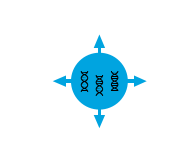
\includegraphics[height=1.5in]{figures/IC1.png}
        \caption{Non-cancer cell: Normal DNA}
    \end{subfigure}
    ~ 
    \begin{subfigure}[t]{0.45\textwidth}
        \centering
        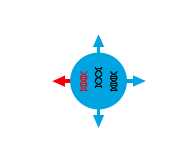
\includegraphics[height=1.5in]{figures/IC2.png}
        \caption{Cancer cell: Mutated DNA}
    \end{subfigure}
\end{figure}
\end{frame}
\begin{frame}{Immunotherapy Enables the Immune System}
The immune system is extremely good at fighting cancer. Immunotherapy 'releases the brakes' on the immune system in order that it can attack tumours.
\begin{figure}[t!]
    \centering
    \begin{subfigure}[t]{0.45\textwidth}
        \centering
        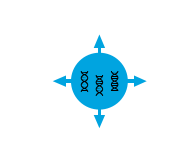
\includegraphics[height=1.5in]{figures/IC1.png}
        \caption{Low-damage cell: Unrecognisable to immune system}
    \end{subfigure}
    ~ 
    \begin{subfigure}[t]{0.45\textwidth}
        \centering
        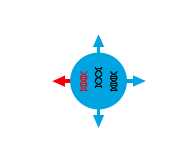
\includegraphics[height=1.5in]{figures/IC2.png}
        \caption{High-damage cell: Recognisable to immune system}
    \end{subfigure}
\end{figure}
However, the immune system can only attack tumours that it recognises!
\end{frame}

\subsection{Exome-Wide Biomarkers}

\begin{frame}{Estimating Tumour Mutation Burden}
As a simplest proxy for likelihood of immune response, we can use tumour mutation burden:
\[
T = \sum_{g \in G} M_g
\]
where $G$ is the collection of genes in the genome, and $M_g$ is the number of mutations in gene $g$. \\
~\\
We want an estimator $\hat{T}$ that relies on observation of only some of the $M_g$s. For example in the case of a linear estimator, we may want 
\[\hat{T} = \sum_{g \in G} w_g M_g \]
with the coefficients $w_g$ sufficiently sparse.
\end{frame}

\subsection{Pratical Restrictions}

\begin{frame}{Liquid Biopsy and Cheap Sequencing}
We have two main restrictions in the data available:
\begin{enumerate}[I]
    \item Liquid biopsy: we only have access to DNA sequencing data!
    \item Cheap sequencing: we only have access to some of that! (but we can choose)
\end{enumerate}
\end{frame}


\section{Generative/Predictive Model Framework}
\begin{frame}{Generative Models of Mutation}
In order to realise the procedure above we need two things:
\begin{enumerate}[I]
    \item A generative model: a suitable joint distribution for the $M_g$s. 
    \item A predictive procedure: a means of getting from the learned generative model to predictions on unseen samples.  
\end{enumerate}

\end{frame}

\begin{frame}{Generative Models of Mutation}
In order to realise the procedure above we need two things:
\begin{enumerate}[I]
    \item A generative model: a suitable joint distribution for the $M_g$s. 
    \[\mathrm{E.g.} \quad M_g \sim \mathrm{Poisson}(\lambda_g)\]
    \item A predictive procedure: a means of getting from the learned generative model to predictions on unseen samples.
    \[\mathrm{E.g.} \quad \min_{\hat{T}}\{\mathbb{E}[(T-\hat{T})^2] + \lambda|\hat{T}|\}\]
\end{enumerate}

\end{frame}

\section{Application to Non-Small Cell Lung Cancer}

\end{document}